\section{System Level and SystemC-PPA}
\label{sec:system-level}
The system-level model is executable. %
It is composed of modules that communicate with each other. %
Communication is modeled on the transaction level, i.e., the system
behavior is that of time-abstract and world-level descriptions of
finite state machines sending each other messages based on
synchronization events. %
Each module is modeled as a PPA describing the behavior as an FSM in
terms of its I/O states and transitions. %
The behavior at the system level results from an \emph{asynchronous
  product} of the individual FSMs. %
This allows for a modeling of all interleavings of messages being
passed between the modules, and ensures capturing the full behavior of
the system-level model. %
Due to the untimed behavior of the system-level model, each module is
allowed to run at its own speed. %
In order to exchange a message between two modules they need to
synchronize through a handshake. %

At system level this handshake is implemented through events. %
During the RTL design process the handshake is realized by a
four-phase handshake. %

Sometimes, implementing full four-phase handshaking bears unnecessary
overhead, e.g., in cases where loosing a message is acceptable. %
\SYSTEMCPPA{}, therefore, provides three different kinds of
communication interfaces called \emph{ports}. %
The three supported interfaces, in our experience, provide enough
flexibility to handle any hardware communication needs. %
The type of communication interface is selected during the
system-level design process. %

Each interface generates a different kind of property suite and,
therefore, affects the hardware design process. %
The basic interface is called \textit{blocking} and implements a
blocking message passing handshake. %
It ensures that a message is never lost. %
\textit{MasterSlave} is a special case of the blocking interface for
synchronous communication. %
If it is known that one side (the \emph{slave}) is always ready for
communication then the other side (\emph{master}) may communicate
without waiting for synchronization. %
Finally, the \textit{Shared} interface models the behavior of a
volatile memory. %

In order to simulate and verify the system-level design an executable
description of the system is needed. %
The industry standard for executable system-level designs is SystemC,
but the semantics of SystemC do not match the semantics of our formal
model perfectly. %
SystemC, as well as many other high-level modeling languages employed
in industry, are primarily software programming languages. %
For example, SystemC is used by a framework of class hierarchies and
macro definitions to describe the structure of hardware systems, with
the associated behavior being modeled in C++. %
While C++ has clearly defined semantics as a programming language, the
high-level objects defined in the SystemC class framework lack precise
semantics with respect to the abstract hardware designs they are
intended for. %
We solved this by restricting SystemC to a subset of certain
constructs called SystemC-PPA. %

The following example provides an idea on the semantic understanding
of the system-level model for blocking message passing. %
Assuming the component to design is a CPU, most designers will
describe a CPU as a set of modules e.g., ALU, RegisterFile, Control
Unit., which are connected to each other via ports. %
For example, the \textit{Control Unit} has an output port
\tsCODE{next\_instruction} and the \textit{ALU} has an input
\tsCODE{next\_instruction}. %
The \textit{Control Unit} sends a new instruction, formalized as a
message (e.g., \tsCODE{ADD~rs1,~rs2,~rd}), to the \textit{ALU}. %
If the \textit{ALU} is still busy with a different instruction the
\textit{Control Unit} is blocked until the \textit{ALU} is ready for
the next instruction. %
The blocking message passing handshake is sometimes also referred to
as \textit{Rendezvous communication}. %
(Rendezvous communication is an analogy: %
In order for two people to communicate they have to be at the same
place at the same time. %
If either one is missing the other one has to wait.) %

\subsection{Modules}
Listing~\ref{lst:Example-SystemC} shows the code of a SystemC
module. %
It is composed of the constructor, ports, variables and the method
containing the behavior named \textit{fsm()}. %
These constructs are sufficient to describe any abstract hardware
model. %
Every C++ construct not mentioned in this document is not part of the
subset and will be detected as unknown by the tool. %
In the following sections each element is discussed in more detail. %

\begin{lstlisting}[language=C++,
caption={Example of a SystemC module},
label={lst:Example-SystemC},
numbers=left,
captionpos=b,   
basicstyle={\footnotesize},
xleftmargin=5.0ex]
struct Example: public sc_module{
  // Constructor
  Example(sc_module_name name):
    var(9){SC_THREAD(fsm);}
  SC_HAS_PROCESS(FPI_Master);
  
  // Ports
  blocking_in<int> b_in;
  shared_out<bool> s_out;
  
  // Variables
  int value;

  // FSM
  void fsm();
}
\end{lstlisting}
As part of the SystemC library macros for generating modules and
constructors are provided. %
The designer is free to implement the modules with or without using
these macros. %
Listing~\ref{lst:Example-SystemC2} uses the provided macros
\tsCODE{SC\_CTOR} and \tsCODE{SC\_MODULE}, where as
Listing~\ref{lst:Example-SystemC} uses standard C++ class and and
constructor definitions. %

\begin{lstlisting}[language=C++,
caption={Example of a SystemC module},
label={lst:Example-SystemC2},
numbers=left,
captionpos=b,   
basicstyle={\footnotesize},
xleftmargin=5.0ex]
SC_MODULE(Example){
  //Constructor
  SC_CTOR(Example):
    var(9){SC_THREAD(fsm);}
  [...]
}
\end{lstlisting}

\subsection{Variables and Data Types}
If a module requires variables for its behavioral description, they
have to be declared as part of the SystemC module. %
The declaration of local variables within the behavioral description
is not allowed. %
The initial value is set within the constructor's initialization list
and the allowed datatypes for variables are the built-in types:
\textit{bool}, \textit{int} and \textit{unsigned int}. %
Line~12 in Listing~\ref{lst:Example-SystemC} shows the declaration of
an integer variable called \textit{value}. %

The designer is also allowed to use enums or define custom
datatypes. %
The enum has to be defined within the scope of the module, as shown in
listing~\ref{lst:variables} on line~2. %
Line~9 demonstrates the declaration of an enum variable. %
Custom data types are declared as a struct with no constructor and no
methods, as shown in line~4. %
They are called \textit{compound data types}; their members consist of
built-in data types and enums. %
For example, \textit{Msg\_type} defines a compound with three
sub-variables \textit{addr}, \textit{data} and \textit{mode}. %
Every variable defined within the class will be added to the abstract
model. %
The custom data types are added to the abstract model as data types. %
The template generator prints them as a record type in VHDL. %

In the current version of \DeSCAM{} it is not possible to assign an initial value to the sub-variables of a compound type. %
This will be fixed in a future version. % 

\begin{lstlisting}[language=C++,
caption={Variables and custom types},
label={lst:variables},
captionpos=b,   
numbers=left,
basicstyle={\footnotesize},
xleftmargin=5.0ex]
//Enum Data Type 
enum Transfer_mode{read,write};
//Compound Data Type
struct Msg_type{int addr; int data; Transfer_mode mode;}
//Module
struct Example: public sc_module{
  [...]
  //Variables
  Transfer_mode trans_mode;
  Msg_type message;
  //FSM
  [...]
}
\end{lstlisting}

\subsection{Constructor}
\label{section:constructor}

For describing abstract hardware models, the constructor shown in
Listing~\ref{lst:constructor} is sufficient. %
The constructor's initialization list is used for variable
initialization. %
The only allowed parameter is the module name. %
The constructor's body is not taken into consideration. %
More parameters are not needed because the module has to be statically
analyzable. %
Not taking the macro body into consideration is a restriction in the
current version of \DeSCAM{} that will be fixed in the future. %



\begin{lstlisting}[language=C++,
caption={Example of a constructor},
label={lst:constructor},
numbers=left,
captionpos=b, 
basicstyle={\footnotesize},
xleftmargin=5.0ex]
struct Example: public sc_module{
  //Constructor
  Example(sc_module_name name):
    port("port"),
    var(9){SC_THREAD(fsm);}
  SC_HAS_PROCESS(Example);
  [...]
}
\end{lstlisting}

The SystemC macro \tsCODE{SC\_THREAD(fsm)} registers the method
\tsCODE{fsm()} as a thread. 
The macro \\ \tsCODE{SC\_HAS\_PROCESS(Example)} makes the module visible to
the SystemC Scheduler. %
This functionality is purely specific to SystemC and has no meaning
for the abstract model. %
Each port of the module has to be initialized within the constructor
, as shown in line~4. %

\subsection{Ports}
\label{section:ports}
Listing~\ref{lst:ports} demonstrates all of the allowed port types. %
For example, line~4 shows the declaration of a blocking input port
that receives a message of type integer. %
A port declaration always follows the structure
\textit{"interface\_direction $<$message\_type$>$ name;"}. %
Possible interfaces are \textit{blocking}, \textit{shared},
\textit{slave} and \textit{master}, all of which implement a different
blocking mechanism. %
Allowed directions are \textit{in} for receiving and \textit{out} for
sending a message. %
Message types may be any of the built-in types as well as enums and
compound data types.  %
The interface defines how the communication is modeled on the RTL,
hence they play a crucial role in the methodology. %
More detailed discussion follows in section~\ref{section:interfaces}. %

\begin{lstlisting}[language=C++,
caption={Example of all port interfaces},
label={lst:ports},
numbers=left,
captionpos=b,  
basicstyle={\footnotesize},
xleftmargin=5.0ex]
struct Example: public sc_module{
  [...]
  //Blocking interface
  blocking_in<int> blocking_in;
  blocking_out<int> blocking_out;
  //Shared interface
  shared_in<bool> shared_in;
  shared_out<bool> shared_out;
  //Slave
  slave_in<Msg_type> slave_in;
  slave_out<Msg_type> slave_out;
  //Master
  master_in<Transfer_mode> master_in;
  master_out<Transfer_mode> master_out;
  [...]
}
\end{lstlisting}

The following information is for advanced SystemC users. %
This section may be skipped, if the reader desires to use SystemC-PPA, without the need to understand the implementation details. %
A \textit{port} is, actually, an \tsCODE{sc\_port} with a custom interface. %
For example, \tsCODE{slave\_in} is defined as ``\tsCODE{using slave\_in =
sc\_port<slave\_in\_if<T> >}'' and \tsCODE{slave\_in\_if} defines the
interface methods for this port. %

\subsection{Functions}
\label{section:functions}

It is possible to define combinational functions.
These function are regular functions within the class
with the restriction that they are not allowed to change any state variables of the module.
This is ensured by declaring the function \tsCODE{const}.
Obviosly, it is not allowed to declare a \textit{void} return type.
The function may only return built-in datatypes.
Other than that, there are no restrictions.


\subsection{Interfaces}
\label{section:interfaces}

\subsubsection{Blocking}

The blocking interface implements the Rendezvous communication as
mentioned earlier. %
In order to send a message, there are two interface methods
\tsCODE{write(value)} and \tsCODE{nb\_write(value)}. %

By calling \tsCODE{port\_name->write(value)} the sender sends a
message with the specified value and is blocked until the reader is
ready. %

This interface is used for an asynchronous system in order to ensure
synchronization between the modules before message transmission. %
A blocking interface guarantees that a message is never lost. %


In addition to the regular blocking communication mechanism, this 
  interface also allows for non-blocking sending and receiving of
  messages. %
  A non-blocking send is initiated by calling
  \tsCODE{port\_name->nb\_write(value)}. %
  The port sends the message whether the receiver is ready or not, but
  doesn't block the module. %
  If the message is successfully delivered, the function call returns
  \textit{true}. %
  If it is lost, the return value is \textit{false}. %

  Please note that even though this interface is called ``blocking'',
  it contains functions for both, blocking \emph{and} non-blocking
  read and write. %

\begin{wrapfigure}{l}{0.25\textwidth}
  \vspace{-20pt}
    \caption{Transitions for write and nb\_write}
    \label{fig:write-vs-nb-write}
    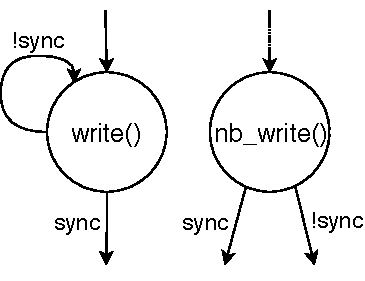
\includegraphics[width=0.25\textwidth]{fig/write_vs_nb_write.pdf}
     \vspace{-40pt}
\end{wrapfigure}

Figure~\ref{fig:write-vs-nb-write} shows the different wait automatons for the regular write and the non-blocking write. %
The Boolean synchronization signal \textit{sync} is \textit{true} 
if the counterpart is ready for communication, \textit{false} otherwise. %
The figure shows the difference in the blocking behavior of those two modules. %

For receiving a message, the methods \tsCODE{read(variable)} and \\ \tsCODE{nb\_read(variable)} are used. %
Upon handshake completion the message sent by the sender is stored in \textit{variable}. %
The receiving interface works similar to the write, with one
difference for the \tsCODE{nb\_read(variable)}:
If no new message is received the value of variable remains unchanged. %

\subsubsection{Shared}

The shared interface offers two methods:
\tsCODE{port\_name->set(value)} for sending a message, and \\
\tsCODE{port\_name->get(value)} for retrieving a message. %
This interface doesn't implement any handshaking mechanism and therefore, is able to model the behavior of a volatile memory. %
The input and output of these ports may change at any time point. %
This interface is needed mainly to model unordered input data like
sensor values. %

For example, if a value from an analog-digital converter is read, a
handshaking mechanism is not necessary because the value changes
continuously and the system reads whatever value is present at the
current time point. %
The same idea applies for sending a value to a peripheral device. %

Because the interface doesn't implement a handshaking mechanism there
is no wait state necessary for using a shared port. %
The shared ports become part of the datapath and are internally
treated like variables that are visible from the outside/inside. %
Hence, the shared ports are going to show up in the datapath of the
generated properties. %

\subsubsection{MasterSlave}

This is a special interface that is only allowed to be used in
\emph{synchronous} hardware systems, i.e., systems using a common
clock. %
The interface is split into two sides, the \emph{master} side and the
\emph{slave} side. %
The common use case for this interface is synchronous communication
between two modules for which the system-level designer knows that a
message sent/received by a master cannot be lost because the
corresponding slave is always ready to communicate. %
This behavior is enforced by the properties generated later for this
construct. %

\begin{lstlisting}[language=C++,
caption={Example of all port interfaces},
label={lst:ports_interface},
numbers=left,
captionpos=b,  
basicstyle={\footnotesize},
xleftmargin=5.0ex]
struct Example: public sc_module{
  [...]
  master_in<Transfer_mode> master_in;
  master_out<Transfer_mode> master_out;
  [...]
}
\end{lstlisting}

Each master has to be connected to a slave. %
The master interface offers the \tsCODE{port\_name->write(value)}
method for sending and \tsCODE{port\_name->read(var)} for reading a
message. %
The slave interface offers \textit{void}
\tsCODE{port\_name->nb\_write(value)} for sending and \textit{bool}
\tsCODE{port\_name->nb\_read(value)} for reading a message. %
For the slave\_out port the write method doesn't block, because
possibly loosing the message is accepted and the master is not
required to catch every message. %
For the slave\_in port a nb\_read method is necessary because the
message should only be captured if the corresponding master\_out did
actually send a message. %
The return value of nb\_write is \textit{void}. %
Method nb\_read returns \textit{true} if there is a new message from a
master, and \textit{false} otherwise. %

The semantics of this interface is that the master is allowed to
communicate at any time point with the guarantee that the slave is
always ready. %
No message from a master to a slave is lost and there is always a new
message from a slave to a master. %
The slave accepts loosing a message, for example a \textit{slave\_out}
port writes a message at each time point and accepts that the master
doesn't receive its message. %
A \tsCODE{slave\_in} port always tries to receive a message. %
At the system level the master is blocked until the corresponding
slave is ready for communication whereas the slave modules never
block. %
Once a module has a slave port, it is considered a slave module,
requiring that
\begin{itemize}
 \item every slave port is used within the FSM, 
 \item no slave port is used a second time before every other slave-port has been used, 
 \item the order in which the slave ports are used has to remain the same for each possible execution path, 
 \item no ports with blocking interface may be used if a module
   contains the slave side of a MasterSlave interface. %
\end{itemize}

\subsection{FSM}
\label{section:FSM}

\subsubsection{Basic Features and Example}
\label{sec:fsm-basic}

The supported set of language features allows ESL modeling of
any type of digital hardware. %
The mentioned modeling restrictions may forbid the use of certain SystemC constructs, but they warrant the precise semantics of the models and they are key to enabling a sound top-down refinement. % 

Listing~\ref{lst:behavior} shows the basic structure of the method
describing the behavior. %
When modeling the behavior, the user needs to adhere to the code
structure shown in the example: %
There must be a single function that is registered as the one and only
SystemC thread (cf.~line~5) in this module. %

The function must contain one outer infinite loop written as
\textit{\small while (true) \{ \ldots \}} with the body describing the
behavior, as shown in the example. %
This is necessary to precisely define a finite state control behavior
in the form of a FSM. % %
Because a module only has one possible behavior the user is only
allowed to use one thread for describing the behavior. %
  The use of threads is necessary for simulation of blocking behavior
  (because \tsCODE{sc\_process} and \tsCODE{sc\_method} cannot be
  blocked). %

The continuous operation of digital hardware is modeled by the
infinite \textit{\small while (true)} loop. %
The model describes untimed behavior and thus all notions of time,
except \tsCODE{sc\_zero\_time}, are not allowed. %
\newpage
\begin{lstlisting}[language=C++,
caption={Behavior description},
label={lst:behavior},
numbers=left,
captionpos=b,   
basicstyle={\footnotesize},
xleftmargin=5.0ex]
struct Example: public sc_module{
  [...]
  //FSM
  void fsm(){
      while (true){
      [...] //Functional description here 
      wait(sc_zero_time);
      }
  };
}
\end{lstlisting}

Listing~\ref{lst:example_1} shows a simple behavioral description
providing an overview of allowed constructs within \SYSTEMCPPA{}. %
In line~4, a message from the input port \textit{blocking\_in} is read
by calling the interface method \textit{read()}. %
the value of the message is stored in an integer variable \textit{frames\_ok}. %

\begin{wrapfigure}{l}{.55\textwidth}
\begin{lstlisting}[language=C++,
caption={Example1},
label={lst:example_1},
numbers=left,
captionpos=b,   
basicstyle={\footnotesize},
xleftmargin=5.0ex]
void fsm(){
    while(true){
    //Read blocking port
    blocking_in->read(frames_ok);
    if(framework > 10){
      ++succ_cnt;
      success = blocking_out->nb_write(succ_cnt);
      shared_out->set(success);
    }else succ_cnt=0;
    wait(sc_zero_time);
    }
};
\end{lstlisting}
\end{wrapfigure}

The execution of the thread is blocked until the counterpart sends a
message. %
After the message is received execution continues at line~5. %
If \textit{frames\_ok} is larger than 10, a success counter is
incremented by~1 in line~6. %
At line~7, a message is send over the blocking port
\textit{blocking\_out} using the non-blocking interface. %
The port will offer a handshake to its counterpart. %
If the counterpart is ready to communicate, the Boolean variable
\textit{success} will evaluate to \textit{true} and the message is
passed, otherwise \textit{success} evaluates to \textit{false}. %
The shared output \textit{shared\_out} sets its value to \textit{true}
if the communication was successful. %
If \textit{frames\_ok} is less then \textit{10} \textit{succ\_cnt} is
reset to zero. %
As with all examples in this documentation, a complete 
simulation model is provided in directory \tsCODE{doc/Example1/}. %

The module called \textit{Stimuli} models the simulation environment of the
module \textit{Example1} and is not meant to be RTL-implemented using PDD. %
The modules are connected in \tsCODE{sc\_main.cpp}. %
A more detailed view on the connection is provided in
Sec.~\ref{section:model}. %
In order to build the example, follow the standard approach for
building CMake projects. %

\subsubsection{Advanced Features and Example}
\label{sec:fsm-advanced}


The only allowed control structure within the
\textit{while~(true)}-loop are if-then-else constructs. %
The use of \textit{for} and \textit{while} loops is not allowed,
because in order to generate interval properties covering a finite number of clock cycles %
 each path from a communication function call to the next
communication function call has to consist of a finite number of C
statements. %
Unbounded loops violate this requirement.  %
%
However, we can still model bounded loops using a a \SYSTEMCPPA{}
  construct called \textit{sections}. %

This construct also helps 
structuring the behavior into individual operations. %
The properties generated by \DeSCAM{} will refer to the section names to
ease implementation and debugging. %

For the example, in listing~\ref{lst:example_1}, all generated
properties will have the same name appended by a unique identification
number which may make it difficult to distinguish the individual
properties.
However, if the designer places each communication function call in a
separate section, the generated properties reflect the names of the
section containing the calls. %
This allows to easily identify the described the execution path within
the \SYSTEMCPPA{} description. %

Human designers usually decompose behavior into parts that reflect
subfunctions or operations. %
Consider, for example, a module that waits for a start signal and then
reads a specific amount of messages. %
A designer would probably split the behavior into two parts: %
\textit{idle} and \textit{reading}. %
Listing~\ref{lst:example_2} shows the behavioral description of such a
module. %
This example also shows how to use compound data types. %
The declaration of the type is found in \tsCODE{Example2/types.h} and
an example for accessing the sub-variables is found in
\tsCODE{Example2/Stimuli.h}. %

\begin{lstlisting}[language=C++,
caption={Example2},
label={lst:example_2},
numbers=left,
captionpos=b,   
basicstyle={\footnotesize},
xleftmargin=5.0ex]
    //Sections
    enum Sections{idle,reading};
    Sections section,nextsection;

    //Behavior
    void fsm() {
        while (true) {
            section = nextsection;
            if(section == idle){
                block_in->read(start_of_frame);
                if(start_of_frame) nextsection = reading;
            }
            else if(section == reading) {
                msg_port->read(msg);
                ++cnt;
                if(cnt > 4){
                    nextsection = idle;
                    cnt = 0;
                }
            }
            wait(SC_ZERO_TIME);
        }
    };
\end{lstlisting}


In order to model the idle phase and the reading phase, an enum
``Sections'' and two variables of this enum type are declared in lines
2 and~3 and are initialized with \textit{idle}. %
The execution starts in line~8 and continues with line~10. %
A message of Boolean type is read from port \textit{block\_in}. %
In case a new frame is detected the \textit{section} is changed to
reading, if not the \textit{section} \textit{idle} is executed
again. %
If control is transferred to \textit{section} reading the next statement that is
executed is line~14, which receives a new message. %
Afterwards a counter is increased by one and this is repeated until
the counter is greater than~4. %
In this case all the data has been received and the module waits for the next
\textit{start\_of\_frame}. %
Hence, the module changes to \textit{section} \textit{idle} and
\textit{resets} the counter. %
The next execution of the loop will start with line~10 again. %
  Effectively, lines 9 to~12 implement a \textit{while} loop, and lines 13
  to~20 implement a bounded \textit{for} loop. %
The designer is free to use custom enums within the behavioral
description to his convenience. %
If an enum with name \textit{Sections} and variables \textit{section}
and \textit{nextsection} are used, the tool will recognize this and
store this information for later use. %
Furthermore, designs with many if-then-else constructs
are easier to process for the tool if \textit{sections} are used. %

\newpage
\textbf{Best practice} for writing modules is to have only one
communication per \textit{section}. %
This allows the tool to process large modules with many branches more
easily. %
Furthermore, the name of a generated property is derived from the
\textit{section} in which the communication is described. %
It is also allowed to have \textit{sections} without any
communication. %
%

\DeSCAM{} is able to consider execution paths spanning more than one
section, and guarantees that every possible path starts and ends at a
communication function call. %

If no \textit{sections} are used at all the tool implicitly assumes a
single default \textit{section} called \textit{run}. %
 
\subsection{Model}
\label{section:model}

  Now that we know how to describe the functionality of a single
  module we will look at how to put modules together to a system. %

In order to simulate a network of modules with SystemC, each port of
every module has to be connected with its counterpart. %
The ports are connected through \textit{channels}. %
In SystemC, channels are used to model communication and to implement
protocols. %


In order to run the simulation, SystemC requires a function called
\tsCODE{sc\_main} that is the main function for the system designer. %
Within this main function modules are instantiated and connected with
each other. %
The current version of \DeSCAM{} does not support hierarchical networks. %
Therefore, everything needs to be declared on the top level, which is  \tsCODE{sc\_main}. %

We call the set of module instances and the connecting
channels "Model". %

\begin{lstlisting}[language=C++,
caption={Example1 sc\_main},
label={lst:example_1_main},
numbers=left,
captionpos=b,   
basicstyle={\footnotesize},
xleftmargin=5.0ex]
int sc_main(int, char **) {
    //Generating/Receiving messages
    Stimuli stimuli("stimuli");
    //Module
    Example1 example_module("example_module");
    //Channels
    Blocking<int> blocking_channel2("blocking_channel2");
    Shared<bool> shared_channel("blocking_channel");
    Blocking<int> blocking_channel1("blocking_channel1");

    //Connect example_module output to stimuli input
    stimuli.block_in(blocking_channel1);
    example_module.block_out(blocking_channel1);

    //Connect example_module input to stimuli output
    stimuli.block_out(blocking_channel2);
    example_module.block_in(blocking_channel2);

    //Connect shared ports
    example_module.share_out(shared_channel);
    stimuli.share_in(shared_channel);

    sc_start(); //Start simulation
    return 0;
}
\end{lstlisting}

Line~5 in Listing~\ref{lst:example_1_main} shows the instantiation of
the module ``Example1'' with the instance and variable name
\tsCODE{example\_module}. %
The designer is free to create as many instances of modules as
necessary. %
Each module has its own thread during the simulation. %
Module instances are interconnected through channels.  %
There is a channel for each interface. %
\DeSCAM{} requires that only these channels be used for communication between modules. %

Line~7 shows the declaration of a blocking channel of data type
\textit{int}. %
This channel is used to connect the input port \textit{block\_in} of
module \tsCODE{stimuli} to the outport \textit{block\_out} of module
\tsCODE{example\_module} in lines 12 and~13. %
 With the current version of \DeSCAM{}, it is required that each channel have exactly one input and one
output. %
 The simulation of the system is started by using the macro \tsCODE{sc\_start()}. %
The simulation runs until there are no more executable threads(deadlock), or simulation is terminated, for example by calling \tsCODE{sc\_stop()} within one of the threads. %

%%% Local Variables: 
%%% mode: latex
%%% TeX-master: "binder"
%%% End: 
